
\section{Esercizio 1.2.1}
\label{sec: basilea}

\subsection{Problem Statement}
Considera la seguente somma

\[
\sum_{n=1}^{\infty} \frac{1}{n^2} = \frac{\pi^2}{6} = \lim_{N \to \infty} S(N) \quad \text{con} \quad S(N) = \sum_{n=1}^{N} \frac{1}{n^2}
\]


\begin{enumerate}
    \item Calcolare la somma in precisione singola usando l'ordinamento normale, ovvero iniziando la sommatoria da $n = 1$, poi $2, \dots$ ($n = 1, 2, \dots N$)
    \item Calcolare la somma in precisione singola usando l'ordinamento inverso, ovvero iniziando la sommatoria da $n = N$, poi $n = N - 1 \dots$ ($n = N, \dots 2, 1$)
    \item Studiare la convergenza di entrambi i metodi in funzione di $N$, graficando $|S(N) - \pi^2/6|$
    \item Ripetere i punti 1, 2 e 3 in precisione doppia
\end{enumerate}

\subsection{Premessa Teorica}
Le variabili rappresentate in precisione singola (32 bit) riservano 23 bit alla mantissa, garantendo circa 7 cifre decimali significative. In precisione doppia (64 bit) si hanno invece circa 15-16 cifre significative. Al limite della rappresentazione numerica corrisponde l'errore di arrotondamento (\textit{round-off error}): le operazioni eseguite dal calcolatore conservano questo errore, che viene propagato e influenza la correttezza del risultato.

Il problema richiede di osservare come agiscono gli errori di arrotondamento in funzione della precisione (32-bit, 64-bit). Si propone di risolvere numericamente il calcolo di $S(N)$; il confronto con il valore analitico permette di calcolare l'errore assoluto come:
\[
    \sigma = |S(N) - \pi^2/6|
\]

\subsection{Metodi Numerici e Algoritmi}
È nostro interesse studiare l'effetto dell'arrotondamento al variare di $N$. Ogni termine $\frac{1}{n^2}$ viene valutato imponendo che numeratore e denominatore siano rappresentati nella precisione scelta.

Nella rappresentazione \textit{floating point}, l'operazione di somma dipende dall'ordine di grandezza degli addendi. Quando si sommano numeri molto diversi, il calcolatore deve allineare le mantisse traslando quella del numero più piccolo; se la differenza di ordini di grandezza supera la capacità della mantissa, il contributo del numero minore viene perso.

\noindent L'ordinamento sequenziale con cui procede la somma può essere quindi non indifferente per gli effetti dell'errore di \textit{round-off}, il limite alla precisione è dettato principalmente dalla \textit{machine precision} ($\epsilon_{single} \approx 1.2 \times 10^{-7}, \epsilon_{double} \approx 2.2 \times 10^{-16}$)
\begin{enumerate}

    \item Per l'ordinamento normale (crescente):
    $$
    \sum_{n=1}^N \frac{1}{n^2} = \frac{1}{1^2} + \frac{1}{2^2} + \dots + \frac{1}{N^2}
    $$
    la somma parziale $S(n)$ cresce rapidamente stabilizzandosi vicino a $1.645$. Per $n$ grande, il termine $\frac{1}{n^2}$ diventa trascurabile rispetto a $S(n)$, portando alla perdita di informazione. Esiste un valore di $n$ oltre il quale la somma non aumenta più.

    \item Nell'ordinamento inverso (decrescente), sommiamo prima i termini piccoli tra loro. Questi accumulano una somma parziale che cresce gradualmente, permettendo di conservare cifre significative che andrebbero perse se sommate singolarmente a un valore già grande, risultando in un metodo più preciso per il calcolo della somma (nel confronto per $N$ grande).
\end{enumerate}

\subsection{Risultati e Discussione}
I risultati ottenuti confermano le previsioni teoriche. inoltre l'andamento dell'errore evidenzia una soglia critica di $N$, dettata dalla precisione di macchina $\epsilon$, oltre la quale il comportamento numerico diverge sensibilmente dal modello analitico.

\subsubsection{$\Tilde{N}_N$}
\noindent Nell'ordinamento normale, la somma parziale $S(N)$ tende rapidamente al valore asintotico $S \approx 1.645$. Un nuovo termine $1/n^2$ viene ignorato dal calcolatore quando il suo rapporto rispetto alla somma parziale scende sotto la soglia della precisione di macchina:$$    \frac{1/n^2}{S(n)} < \epsilon \implies \frac{1}{n^2} \lesssim 1.645 \cdot \epsilon$$

\noindent Approssimando $S(n) \approx 1$, definiamo $\Tilde{N}_N = 1/\sqrt{\epsilon}$ come il valore di saturazione. Oltre questo limite, ogni ulteriore termine è troppo piccolo per modificare la mantissa della somma già accumulata; l'errore $\sigma(N)$ smette quindi di decrescere e rimane costante (plateau visibile nei grafici).
\[
    \epsilon \ge \frac{1}{n^2} \implies n \ge \frac{1}{\sqrt{\epsilon}}= \Tilde{N}_N \\
\]
\[
    \implies S(n) = S(\Tilde{N}_N) \\
\]
\[
    \implies \sigma(n) = \sigma(\Tilde{N}_N)
\]
\smallskip



\begin{figure} [H]
    \centering
    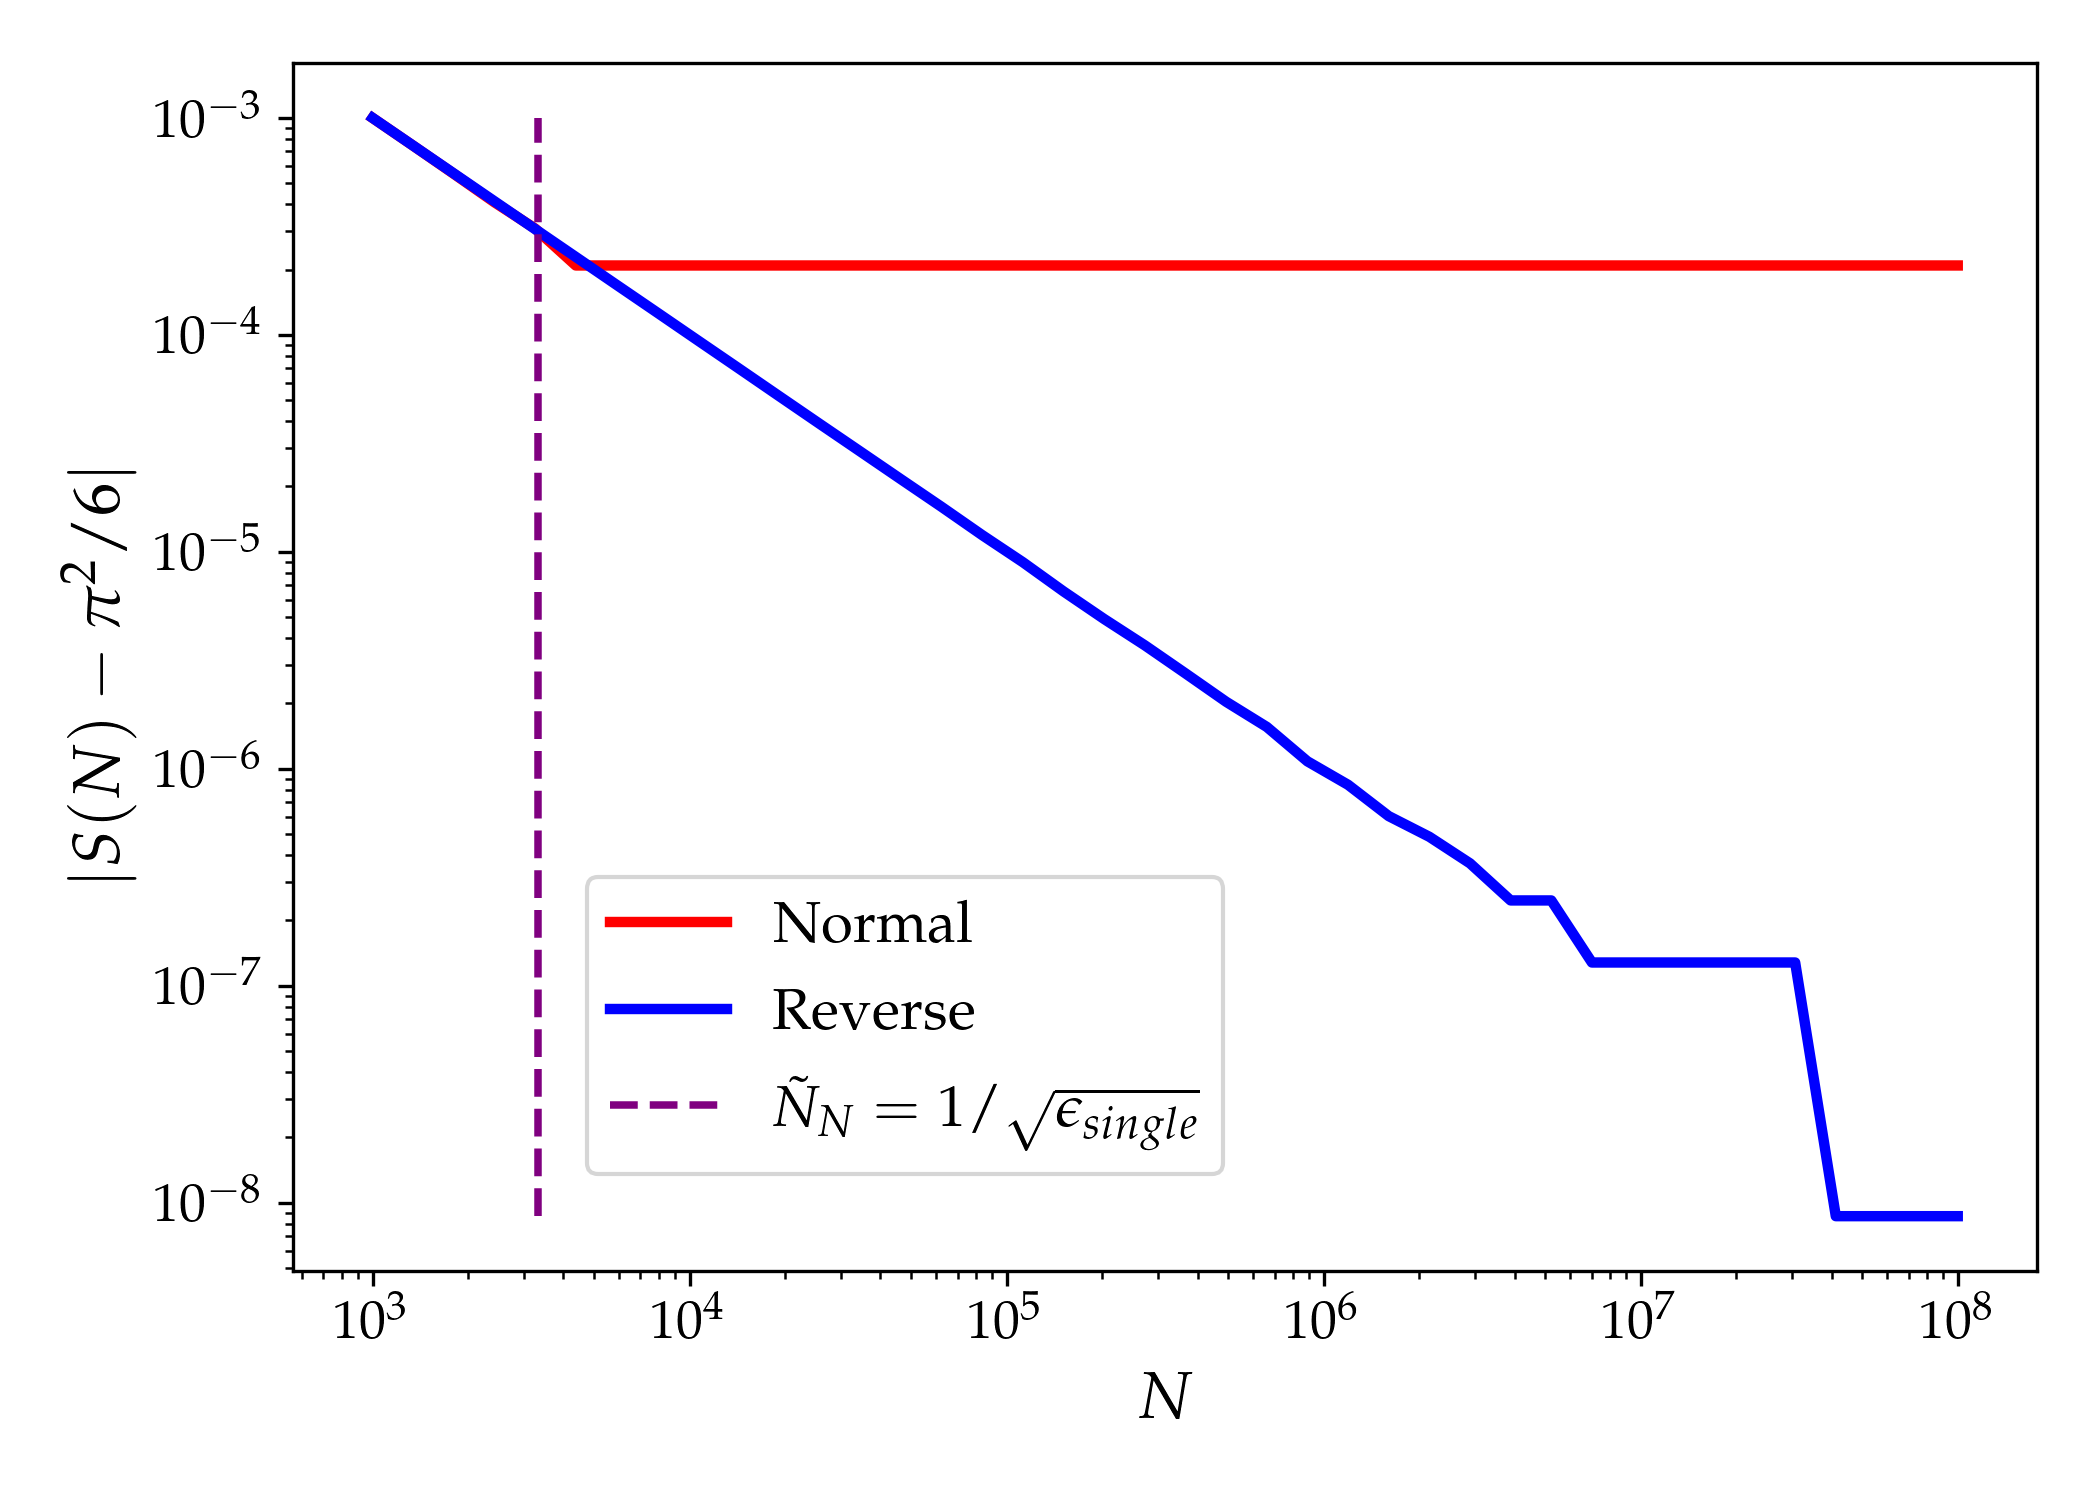
\includegraphics[width=0.7\linewidth]{images/2/SinglePrec.png}
    \caption{Andamento dell'errore assoluto $\sigma(N) = |S(N) - \pi^2 / 6|$ usando lo standard a precisione singola, 32-Bit}
    \label{fig: 1 - single precision}
\end{figure}

\begin{figure} [H]
    \centering
    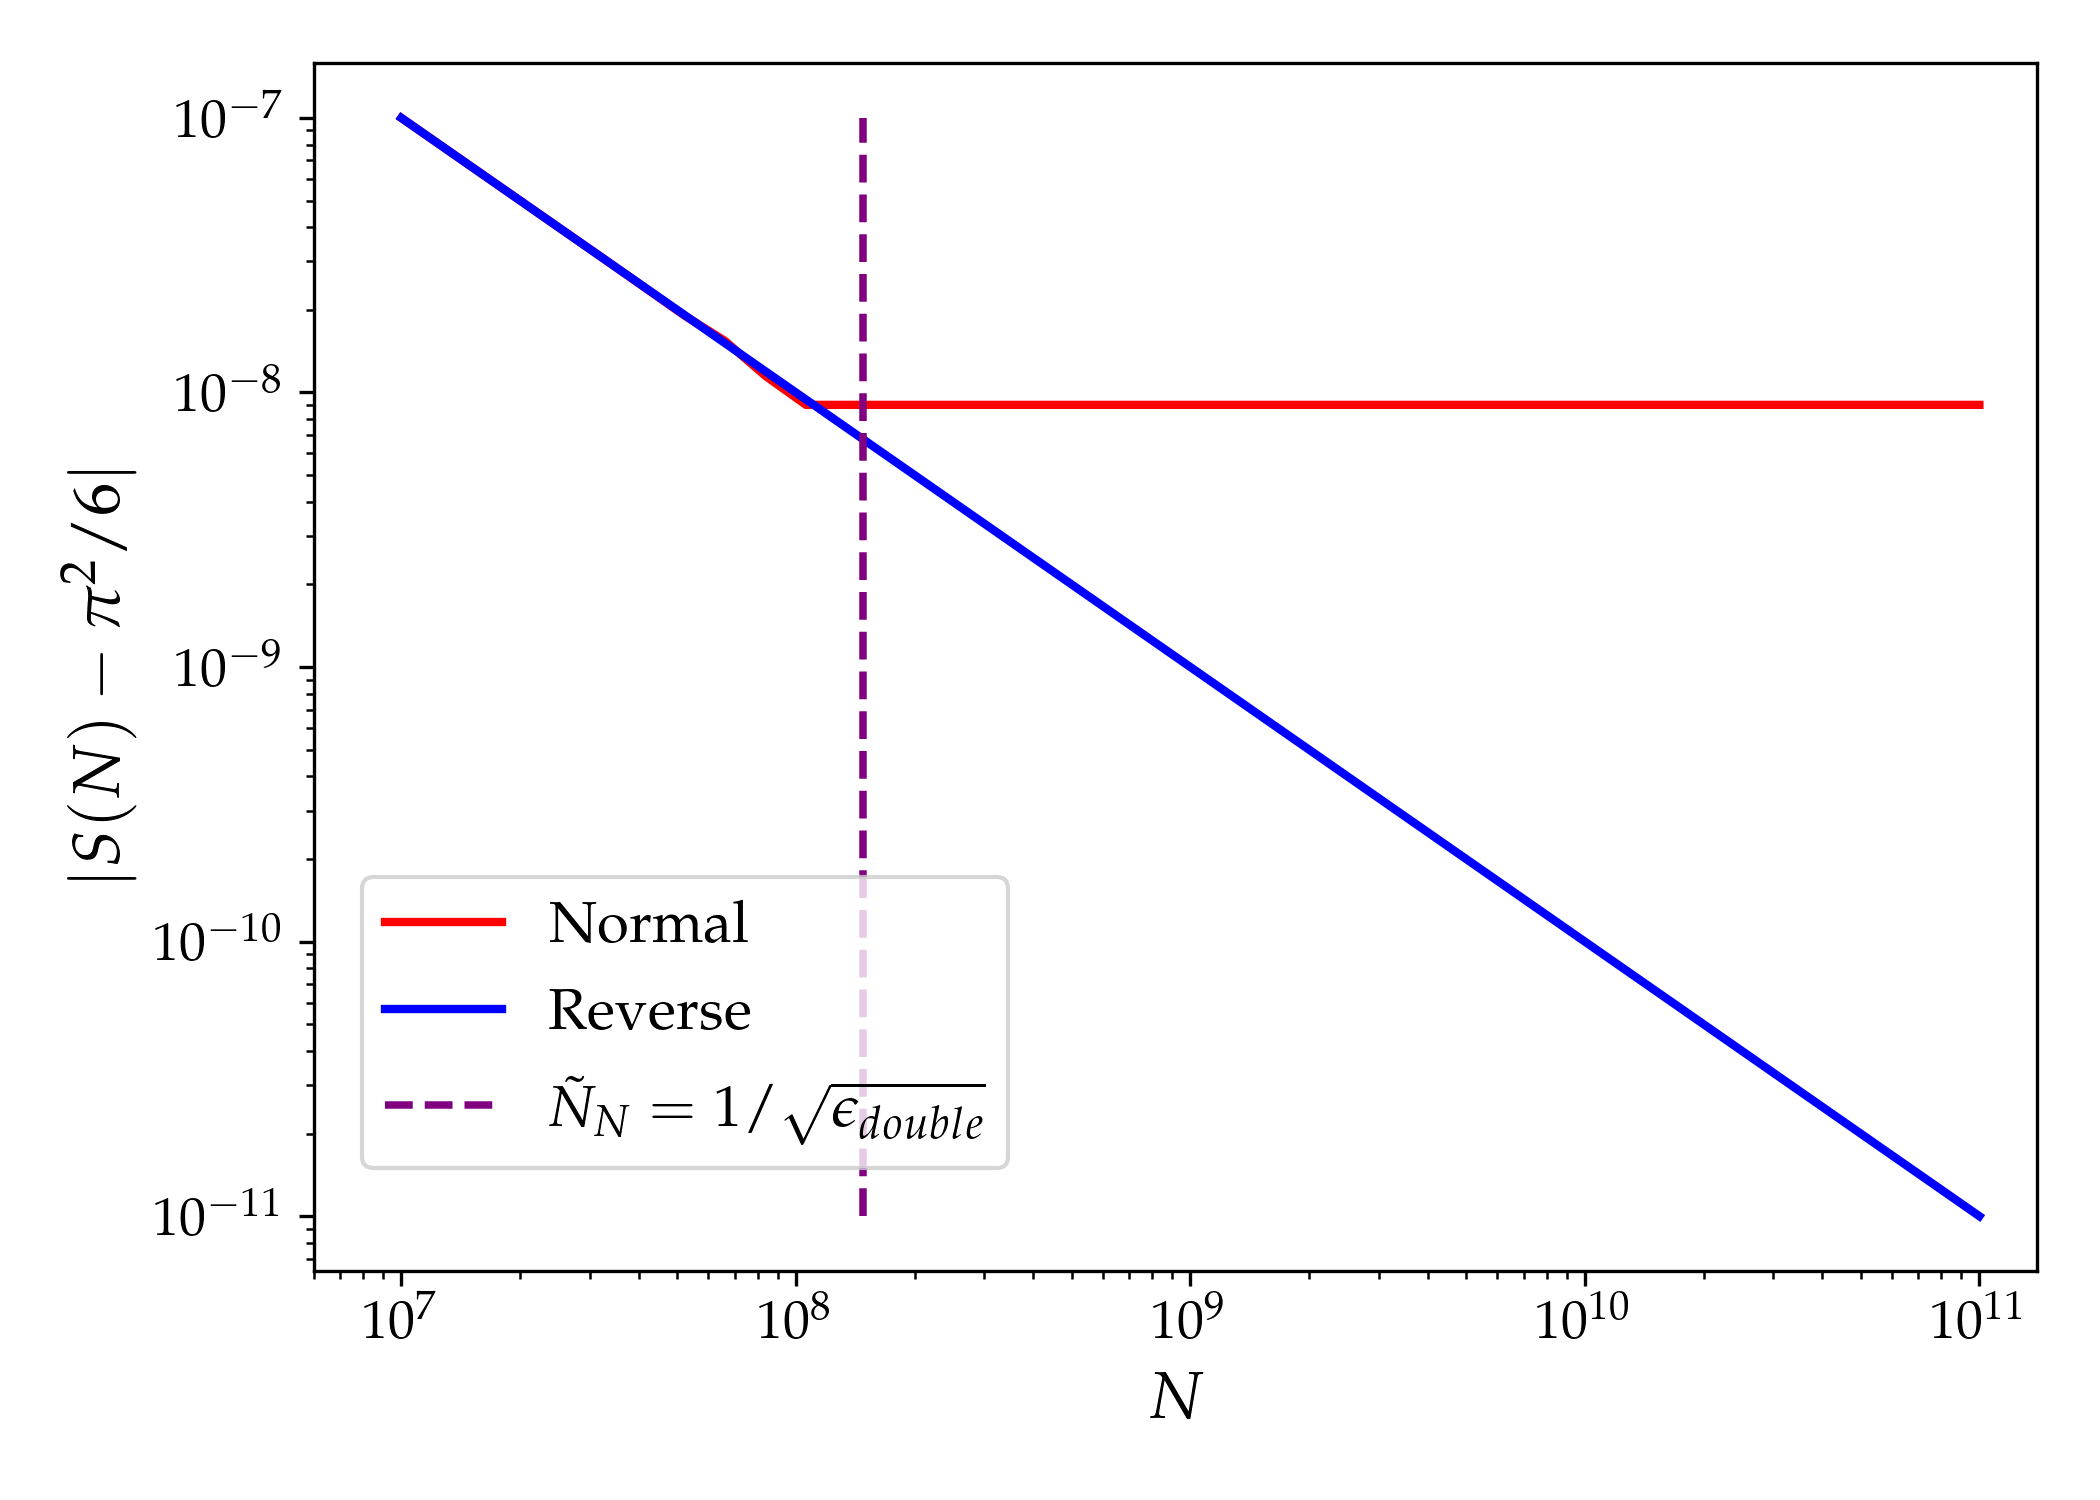
\includegraphics[width=0.7\linewidth]{images/2/DoublePrec.png}
    \caption{Andamento dell'errore assoluto $\sigma(N) = |S(N) - \pi^2 / 6|$ usando lo standard a precisione doppia, 64-Bit}
    \label{fig: 2 - double precision}
\end{figure}
